%% A simple template for a lab or course report using the Hagenberg setup
%% with the standard LaTeX 'report' class

%\documentclass[english,11pt]{report}		
\documentclass[ngerman,11pt]{report}



\usepackage[a4paper, total={6in, 8in}]{geometry}
\usepackage{hgb}
\usepackage{hgbbib}
\usepackage{hgbheadings}
\usepackage{tabularx}
\usepackage{listings}

\graphicspath{{images/}}   % where are the images?
\bibliography{literatur}  % requires literatur.bib 

\author{Andre Wachsmuth}
\title{Programmierprojekt des Moduls Verteilte Systeme \\ Client-Server-Multiplayer-Spiel}
\date{August 2017}

%%%----------------------------------------------------------
\begin{document}
%%%----------------------------------------------------------
\maketitle
\tableofcontents
%%%----------------------------------------------------------

\chapter*{Abstract}

The author implemented a simple online multiplayer game with one server and
multiple clients. Employed technologies are Java Server Faces, HTML5 WebGL, Websockets
and Java Persistence API (Hibernate). The game consists of two scenes, a menu scene and
a battle scene. Each player may own up to 28 characters. Two onlne players must discover each
other mediated by the server and agree to have a battle. The server is responsible for 
managing the game state and game logic, validating messages sent by the client and allow only
valid game states; as well as mediating invitations between players. The Javascript framework
\textit{PixiJs} provides an API for rendering 2D graphics via WebGL and Canvas. It was found
to be efficient and quick to develop with, but does not provide any API for creating user
interfaces or scenegraphs, requiring more programming work.


%%%----------------------------------------------------------
\chapter{Websocket-Kommunikation}
%%%----------------------------------------------------------

Die Kommunikation zwischen Clients und dem Server erfolgt über Websockets. Websocket
sind ein auf \textsc{tcp} basierendes zustandbehaftetes Plain-Text-Protokol, die 
ine bidirektionale Kommunikation für Webanwendungen ermöglicht.

Session-Verwaltung und die Persistierung von Daten während der Session wird von Websockets bereitgestellt.
Der Datenaustausch geschieht mittels Textnachrichten. Zu lösende Probleme sind somit die Authorisierung
von Sessions und die Struktur (Protokoll) der zwischen Client und Server ausgetauschten Nachrichten.

Für die Struktur der Nachrichten wird das \textsc{json}-Format verwendet. Es wird von vielen
Software-Implementierungen unterstüzt. Die zusätzliche Ausdrucksfähigkeit und damit verbundene
Komplexität von \textsc{xml} wird nicht benötigt. Im folgenden wird die \textsc{json}-Struktur
beschrieben. Jede Nachricht beginnt mit der Metanachricht \textsc{lunarmessage}, die folgende
Informationen enthält, siehe hierzu auch Tabelle \ref{table:lunarmessage}.

Der Eintrag status gibt den Verarbeitungsstatus an, dieser ist \textsc{ok} bei korrekter
Verarbeitung. Mögliche Status sind in der Tabelle \ref{table:messagesStatus} zusammengestellt.

Im Eintrag payload werden nachrichtenspezifische Informatione mitgesendet und der Eintrag
type gibt an, um welchen Typ es sich handelt, siehe \ref{table:messageType}. Die Zeichenkette
im Eintrag payload ist ein \textsc{json}-String.

\textsc{tcp} garantiert die Reihenfolge des Nachrichtenempfangs in Reihenfolge des Versandes,
aber nicht die logische Reihenfolge und die Verarbeitung in dieser Reihenfolge durch die
Anwendung. Der Eintrag time dient der Ordnung der Nachrichten. Der Sender setzt bei Beginn
der Websocket-Session einen Laufindex auf null und sendet diesen im Eintrag time bei jeder
Nachricht mit an den Empfänger. Dabei wird der Laufindex bei jeder Nachricht um eins erhöht.
Der Empfänger \textsc{muss} die empfangenen Nachrichten in dieser Reihenfolge bearbeiten.

Jede empfangene Nachricht wird mit einer \textsc{lunarmessage} vom Typ \textsc{received} quittiert,
die den Laufindex nicht erhöht und im payload den Laufindex der quittierten Nachricht enthält.
Diese Nachricht dient beispielweise dazu, dass der Sender die Nachricht aus dem eventuell vorhandenen
implementierungspezifischen Cache löschen kann.
\footnote{Dieser Mechanismus ist derzeit noch nicht implementiert.}

Sind bereits weitere Nachrichten mit höheren Laufindex beim Empfänger eingetroffen und ist ein gewisses
Zeitlimit überschirtten, \textsc{kann} der Empfänger durch Senden einer Metanachricht mit dem
type \textsc{repeat} die Nachricht erneut anfordern. Im Eintrag payload ist der Laufindex der
angeforderten Nachricht enthalten. Der Nachrichtentyp \textsc{repeat} erhöht den Laufindex time nicht.
\footnote{Dieser Mechanismus ist derzeit noch nicht implementiert.}

Der Server reagiert nur auf Nachrichten beziehungsweise informiert den Client über Ereignisse,
erwartet aber keine Antworten. Clients senden immer Nachrichten in Erwartung einer Antwort.
Zur Reduzierung des Programmieraufwandes der Client-Software wurde daher ein
Request-Response-Mechanismus für Nachrichten des Clients implementiert. Alle Nachrichten, deren
type auf \textsc{response} endet, enthalten im payload-\textsc{json} den Eintrag origin, der
den Laufindex der Nachricht enthält, auf die geantwortet wird.

Clients werden bereits vor dem Aufbau der Websocket-Verbindung mittels einer Login-Eingabemaske
auf der Webseite authorisiert. Dabei wird ein zeitbegrenztes Token erstellt und dem Client
übermittelt. Initial wird beim Öffnen einer Websocket-Session diese als unauthorisiert markiert
und bis auf \textsc{authorize} keine anderen Nachrichten akzeptiert. Das Token und der Nutzername wird in
der \textsc{authorize}-Nachricht an den Server übermittelt, der mit \textsc{authorize\char`_response} antwortet.
Bei erfolgreicher Authorisierung wird die Session als authorisiert markiert und der Statuscode \textsc{ok}
übermittelt, \textsc{generic error} andernfalls.

%%%----------------------------------------------------------
\chapter{Server}
%%%----------------------------------------------------------

\section{Eingesetzte Technologien}

Auf dem Server wird \textsc{jsf} (Java Server Faces) eingesetzt, konkreter
Primefaces\footnote{https://www.primefaces.org/ Eine Übersicht über alle
Funktionionen ist unter https://www.primefaces.org/showcase/ zu finden.}.
Das System kann auf verschiedenen Servlet-Containern laufen, zur Entwicklung
wurde Tomcat 8.5 genutzt.

Um periodische Aufgaben auszuführen, wird der
Quartz-Scheduler\footnote{http://www.quartz-scheduler.org/} eingesetzt.

Die Persistierung von Daten nutzt eine Datenbank. Aus Zeitgründen wird ein ORM
(Object Relational Mapping) genutzt, konkret \textsc{jpa} (Java Persistence API)
mit Hibernate\footnote{http://hibernate.org/} als JPA-Provider. Weiterhin wird
HikariCP\footnote{https://github.com/brettwooldridge/HikariCP} eingesetzt, um
Verbindungen zur Datenbank zu verwalten. HikariCP stellt einen Pool an
aufrechgehaltenen Datenbankverbindungen bereit, sodass nicht für jede Anfrage
eine Verbindung geöffnet werden muss.

Das \textsc{erm} für das \textsc{orm} ist in der Abbildungen zu finden. Die Hauptentität
ist die Entität \textsc{player}, welche Assoziatonen auf die \textsc{item}s und
\textsc{characterstate}s des Spielers hat. Diese Informationen werden bei Beginn der
Session aus der Datenbank geladen und zwischengespeichert, um unnötige Datenbankanfragen
zu vermeiden.

\textsc{item}, \textsc{character}, \textsc{item} sind immutable Entitäten, diese Daten
werden einmalig bei der Installation in die Datenbank eingespielt. \textsc{player} und
\textsc{characterstate} sind mutabel und werden öfters im Laufe des Programms geändert.

Der Server ist für die Logik und die Konsistenz der Daten verantwortlich und muss davon
ausgehen, dass es böswillige Client geben kann, demgemäß müssen alle Eingaben und Nachrichten
validiert werden. Dies bedeutet auch, dass die Client-Software nicht für Datenkonsistenz
verantworlich ist, was den Programmiertaufwand reduziert.

Schließlich seien noch kurz weitere eingesetzte Bibliotheken erwähnt: Google
Dagger\footnote{https://github.com/google/dagger} für Dependency Injection,
Jsoniter\footnote{http://jsoniter.com/} für die Serialisierung und
Deserialisierung von Objekten, slf4j für Logging.

\section{Servlets}

Die eingesetzten clientseitigen Technologien erfordern, dass mediale Ressourcen mittels
als \textsc{http}-Response ausgeliefert werden. Es gibt statische und dynamische Inhalte.
Erstere können direkt über den Servlet-Container bereitgestellt werden. Dynamische Inhalte
wie beispielsweise Grafiken der Charaktere, über die der Spieler momentan verfügt, können
nicht statisch ausgeliefert werden. Hierzu gibt es zwei \textsc{http}-Servlets.

Das Resourcen-Servlet stellt Dateien bereit, die dynamisch in der Datenbank gespeichert sind.
Die Dateien werden nicht durch den Nutzer bereitgestellt und liegen somit in der Kontrolle des
Programmierers beziehungsweise des Administrators. Zudem ist keine hierarchische Gliederung
der Dateien notwendig. Daher wurde ein einfaches Datenbankschema mit einem eindeutigen Namen
als primärer Schlüssel gewählt. Es muss darauf geachtet werden, keine doppelten Namen zu nutzen.

Das Spritesheet-Servlet erlaubt das Abholen mehrerer Dateien mit einem \textsc{http}-Request.
Ziel ist es, zu vermeiden, dass clientseitig bis zu fünfzig und mehr kleinere Bilddateien im
KiB-Bereich angefordert werden müssen. Dazu wird serverseitig eine große Bilddatei generiert,
die die kleineren Bilder enthält und serverseitig in einem Cache gehalten.
In einer dazugehörigen \textsc{json}-Datei ist festgehalten, an welcher Position sich jedes Bild befindet. Der Client fordert zuerst das \textsc{json} an und anschließend die Bilddatei. Der Cache
dient dazu, bei der zweiten Anforderung die Bilddatein nicht erneut generieren zu müssen und die
Einträge haben daher eine kurze Lebensdauer.

%%%----------------------------------------------------------     
\chapter{Client}
%%%----------------------------------------------------------

Die Clientsofware wurde in JavaScript (ES6) und läuft in einem Webbrowser. Dieses wird
mittels babel\footnote{https://babeljs.io/} transpiliert, sodass die Software auch mit
älteren Browsern kompatibel ist. Dazu wird auch wird auch
polyfill\footnote{https://babeljs.io/docs/usage/polyfill} eingesetzt. Die Aufgabe des Clients
besteht in der grafischen Darstellung des Programmzustands zur Nutzerinteraktion und
Weiterleitung der Nutzereingaben an den Server. Die Architektur wurde einfach gehalten,
es gibt eine Komponente für Netzwerk und generelle Aufgaben, sowie Komponenten für die
einzelnen dargestellten Spieleszenen. Dies ist auch in Abbildung \ref{fig:clientarch} dargestellt.

Es wurde eine generische Methode \textit{dispatchMessage} der Klasse \textit{Lunar.Net} (Datei \textit{010-net.js} geschaffen, welche analog zu \textsc{jQuery.ajax} die Websocket-Netzwerkkomunikation
abstrahiert:

\begin{lstlisting}
Lunar.Net#dispatchMessage(Lunar.Message message, object payload) : Promise
\end{lstlisting}

Es wird der Nachrichtentyp und der zu sendende Inhalt als Javascript-Objekt übergeben. Mittels
des zurückgegebenen \textit{ES6-Promise} kann asynchron Logik ausgeführt werden, wenn der Server
auf die gesendete Nachricht antwortet und auch der Fehlerfall entsprechend behandelt werden (\textit{Promise.catch}.

Ein interaktives Spiel erfordert Nutzereingaben. Pointereingaben (Maus, Touch-Screen) ist problemlos möglich. Bei Texteingaben ist es möglich, diese mittels Abfragen der Tastatur nativ in Canvas beziehungsweise WebGL zu implementieren. Hierfür existieren auch bereits einige Bibliotheken. Allerdings musste ich feststellen, dass diese nur begrenzte Eingabemöglichkeiten erlauben, speziell in Bezug auf Eingabemethoden und mobile Geräte habe ich Mängel bemerkt. Daher wurden Eingaben mittels nativer HTML-Input-Elemente umgesetzt, die mittels \textit{z-order} überhalb des Canvas platziert werden. Optisch können diese Input-Elemente mittels \textsc{css} and das Layout angepasst werden, allerdings kann kein Gradient für die Textfarbe eingstellt werden.

Für die grafische Darstellung wird die Bibliothek PixiJS\footnote{http://www.pixijs.com/}
verwendet, die \glqq The HTML5 Creation Engine\grqq. PixiJS nutzt \textsc{WebGL} mit
Fallback auf Canvas, wenn \textsc{WebGL} nicht zur Verfügung steht. Diese Bibliothek
wurde gewählt, da sie aktuell und lightweight ist sowie  eine gute Dokumenation mit
Beispielen besitzt.

Für die Ausgabe von Audio wird die Bibliothek HowlerJS\footnote{https://howlerjs.com/}
verwendet. Diese Bibliothek unterstützt alle gängigen Formate mit Fallbacks. In
diesem Projekt wird das Format \textit{webm} mit Fallback auf \textit{mp3} verwendet, dies
wird von allen moderenen Browser unterstützt\footnote{https://github.com/goldfire/howler.js}.



%%%----------------------------------------------------------     
\chapter{Einrichtung und Installation}
%%%----------------------------------------------------------

Die Installation des Systems erfordert einen Server (Servlet Container) sowie
eine von Hibernate unterstützes Datenbanksystem. Weiterhin müssen die Datenbankeinstellung
konfiguriert werden und Initialdaten eingespielt werden.

Application Server. Es muss Java 8 und JSF 2.1+ unterstützt werden. Während der Entwicklung wurde
Apache Tomcat 8\footnote{http://tomcat.apache.org/download-80.cgi} genutzt und auch mit diesem
getestet. Es wurde keine spezifischen Funktionen des Tomcat genutzt, sodass auch andere Servlet
Container genutzt werden können, dies wurde aber nicht getestet.

Datenbanksystem. Das Datenbanksystem muss von Hibernate unterstützt werden.\footnote{Inbesonders unterstützt werden PostgreSQL MySQL Microsoft SQL, Oracle. Nicht unterstützt wird SQLite.} Weiterhin muss das Datenbanksystem
in der Datei \textit{hibernate.cfg.xml} konfiguriert werden.\footnote{Standardformat von Hibernate. Siehe etwa https://docs.jboss.org/hibernate/orm/3.3/reference/en/html/session-configuration.html, Abschnitt 3.7} In der
mitgelieferten Datei ist bereits eine beispielhafte Konfiguration für MySQL und MariaDB vorhanden.

Nach Starten des Application Servers und dem Deployment der Anwendung kann die Nutzeroberfläche im Webbrowser
im Context Path aufgerufen werden.\footnote{Zum Beispiel bei lokaler Ausführung \textit{http://localhost:8080/translune}}. Es erscheint eine
Eingabemaske für das Login. Bereits registrierte Nutzer können sich hier mit ihrem eindeutigen Nutzernamen
und Passwort anmelden. Mit dem Nutzernamen \textit{sadmin} und Passwort \textit{sadmin} kann eine einfache
Verwaltungsoberfläche betreten werden. In der Datei \textit{custom.properties} ist das Administratorpassword
als SHA1-Hash gespeichert und kann dort geändert werden. 

In der Administratoroberfläche muss unter Verwaltung das Paket mit den Initialdaten eingespielt werden. Dabei
handelt es sich um eine gepackte Datei im \textsc{zip}-Format und enthält die in Tabelle \ref{table:initdata}
dargestellten Dateien und Ordner.

%%%----------------------------------------------------------     
\chapter{Optimierungspotential}
%%%----------------------------------------------------------

Derzeit existiert keine Lastenverteilung, alle Anfragen werden von einem Server bearbeitet.

Bei Analyse des Domain Object Model fällt auf, dass sich Entitäten in statische und dynamische
trennen lassen. Die statische Entitäten \textit{Resource}, \textit{Item}, \textit{Character}
und \textit{Skill} werden bei der Einrichtung des Systems angelegt und ändern sich während der
Laufzeit nicht. Durch diese Immutabilität ist zwischen Servern keine Synchronisation erforderlich.
Die dynamischen Entitäten sind \textit{Player} mit den dazugehörigen \textit{CharacterState}.

Für \textit{Player} Es können mehrere Server eingerichtet werden, welche jeweils die Websocket-Sessions eines Teils der \textit{Player} übernehmen. Diese Server müssen miteinander kommunizieren können.
Hierbei ist das Synchronisationsproblem zu lösen, wenn ein Server Daten eines \textit{Players} auf
einem anderen Server benötigt. Dies kann mittels \textit{Push} oder \textit{Poll} gelöst werden.
Im ersten Fall übermittelt ein Server bei Änderungen an einem von ihm verwalteten \textit{player}
diese an die anderen Server im Verband. Dabei muss über einen geeingeten Mechanismus sichergestellt
werden, dass alle Server die Nachricht erhalten haben. Im zweiten Fall fragt ein Server nach den
Daten bei Bedarf bei dem enstprechenden Server Daten nach. Diese Möglichkeit ist sicherer, 
weist allerdings einen höheren Kommunikationsbedarf auf.

Bei der Entität \textit{Resource} handelt es sich um herunterladbare Binärdaten. Sie ist zudem
unabhängig von anderen Entitäten. Für die Bereitstellungen von \textit{Resourcen} kann mithin
ein separater Provide-Server erstellt werden.

Auf Seite des Clients kann versucht werden, die Anzahl der Websocket-Frames zu reduzieren, um
die Server-Last zu reduzieren und die Ladezeiten gering zu halten. Dies kann durch Bündelung einiger
Nachrichten erreicht werden, dies schränkt aber die gute Strukturierung des Programmes ein.

Es wurden keine Lasttests durchgeführt.

%%%----------------------------------------------------------     
\chapter{Anhang}
%%%----------------------------------------------------------

\begin{table}[]
\centering
\caption{Einträge der \textsc{json}-Struktur der Metanachricht \textsc{lunarmessage}}
\label{table:lunarmessage}
\begin{tabularx}{\textwidth}{l|l|X}
Eintrag & Datentyp & Erläuterung \\ \hline
time    & int    & Eine bei null beginnende Ganzzahl. Dient der Synchronisation der Nachrichten. \\
type    & string & Art der Nachricht, gibt an, wie der Eintrag payload interpretiert wird  \\
status  & int    & Verarbeitungsstatus, beispielweise 0 für \textsc{ok}                          \\
payload & string & Typenspezifische Nachricht. Enthält einen \textsc{json}-String.       
\end{tabularx}
\end{table}


\begin{table}[]
\centering
\caption{Mögliche Verabeitungsstatus in der Metanachricht \textsc{lunarmessage}}
\label{table:messagesStatus}
\begin{tabularx}{\textwidth}{l|l|X}
Bezeichnung            & Wert & Erläuterung \\ \hline
\textsc{ok}            & 0    & Fehlerfreie Verarbeitung. \\
\textsc{generic error} & 20   & Nicht näher spezifizierter Fehler in der Verarbeitung.  \\
\textsc{access denied} & 21   & Fehlende Authorisierung. Zur Authorisierung muss die
                                Nachricht \textsc{authorize} gesendet werden. \\
\textsc{timeout}       & 22   & Überschreitung des Zeitlimits bei der Verarbeitung.
\end{tabularx}
\end{table}


\begin{table}[]
\centering
\caption{Ordnerstruktur des Intialdatenarchivs (\textsc{ZIP}-Archiv)}
\label{table:initdata}
\begin{tabularx}{\textwidth}{l|1|X}
Pfad & Typ & Erläuterung \\ \hline
skills.csv      & CSV & Fähigkeiten der Charaktere \\
chars.csv       & CSV & Daten vorhandener Charktere \\
chartoskill.csv & CSV & Tabelle mit erlernbaren Fähigkeiten der Charaktere \\
character-cry   & Ordner & Enthält SFX für Charaktere. Muss jeweils mit Dateiendung \textit{webm} und \textit{mp3} vorliegen. Der Dateiname ist im Feld \textit{cry} der \textit{chars.csv} definiert. \\
character-icon  & Ordner & Enthält Icons der Charaktere. Sollte  im \textit{png} vorliegen. Dateiname mit Dateiendung ist im Feld \textit{imgIcon} der \textit{chars.csv} definiert. \\
character-img  & Ordner & Enthält Spritesheets der Charaktere. \textit{json}-Format von PixiJS/TexturePacker\footnote{https://www.codeandweb.com/texturepacker}. Dateiname mit Dateiendung ist im Feld \textit{imgFront} (Vorderansicht) beziehungsweise \textit{imgBack} (Hinteransicht) der \textit{chars.csv} definiert. \\
bg-menu        & Ordner & Enthält vorhandene Hintergründe für die Menuszene. \\
bg-battle      & Ordner & Enthält vorhandene Hintergründe für die Kampfszene. \\
bgm-menu       & Ordner & Enthält vorhandene Hintergrundmusik für die Menuszene. \\
bgm-battle     & Ordner & Enthält vorhandene Hintergrundmusik für die Kampfszene. \\
default        & Ordner & Enthält Fallback-Dateien für nutzerkonfigurierbare Inhalte: Derzeit nur \textit{pavatar.png} für das Nutzeravatar.
\end{tabularx}
\end{table}


\begin{table}
\centering
\caption{Nachrichtentypen im Eintrag payload einer \textsc{lunarmessage}}
\label{table:messageType}
\begin{tabularx}{\textwidth}{l|X}
Bezeichnung & Erläuterung \\ \hline
\textsc{authorize}                           & Authorisierung der Session \\
\textsc{authorize\char`_response}            & Status \textsc{ok}, wenn authorisiert\\
\textsc{fetch\char`_data}                    & Ahbolen von benötigten Daten, beispielweise Daten von Items\\
\textsc{fetch\char`_data\char`_response}     & Antwort mit den angeforderten Daten. \\
\textsc{update\char`_data}                   & Ändern von Daten, beispielsweise einer Beschreibung. \\
\textsc{update\char`_data\char`_response}    & Antwort, ob die Änderung erfolgreich war. \\
\textsc{invite}                              & Einladen eines anderen Spielers \\
\textsc{invite\char`_response}               & Antwort. \\
\textsc{invited}                             & Nachricht vom Server an Client, wenn Einladung von anderem Client vorliegt \\
\textsc{invite\char`_accept}                 & Client lädt einen anderen Client ein \\
\textsc{invite\char`_accept\char`_response}  & Antwort. \\
\textsc{invite\char`_accepted}               & Nachricht vom Server an Client, wenn anderer Client Einladung akzeptiert hat \\
\textsc{invite\char`_retract}                & Client zieht Einladung zurück \\
\textsc{invite\char`_retract\char`_response} & Antwort. \\
\textsc{invite\char`_retracted}              & Nachricht vom Server an Client, wenn anderer Client die Einladung zurückgezogen hat \\
\textsc{invite\char`_reject}                 & Client akzeptiert Einladung nicht \\
\textsc{invite\char`_reject\char`_response}  & Antwort. \\
\textsc{invite\char`_rejected}               & Nachricht vom Server an Client, wenn anderer Client Einladung nicht akzeptiert hat \\
\textsc{prepare\char`_battle}                & Client sendet Kampfkonfiguration \\
\textsc{prepare\char`_battle\char`_response} & Antwort. \\
\textsc{cancel\char`_battle}                 & Client bricht Kampfkonfiguration ab.\\
\textsc{cancel\char`_battle\char`_response}  & Antwort.\\
\textsc{step\char`_battle}                   & Client sendet Kampfzugkonfiguration \\
\textsc{step\char`_battle\char`_response}    & Antwort. \\
\textsc{battle\char`_prepared}               & Nachricht vom Server an beide Clients, wenn Kampfvorbereitung abgeschlossen \\
\textsc{battle\char`_stepped}                & Nachricht vom Server an beide Clients, wenn Kampfzugberechnung abgeschlossen \\
\textsc{battle\char`_cancelled}              & Nachricht vom Server an beide Clients, wenn Kampf abgebrochen wurde \\
\textsc{battle\char`_ended}                  & Nachricht vom Server an beide Clients, wenn Kampfende erreicht wurde \\
\textsc{loot}                                & Client sendet Beuteinformationen \\
\textsc{loot\char`_response}                 & Antwort. \\
\textsc{unknown}                             & Fallback für unbekannte Nachrichten
\end{tabularx}
\end{table}

\begin{figure}
\caption{Entity-Relationship-Model für die Datenstruktur. Persistierung mittels Hiberante. Quelle: eigene Darstellung}
\centering
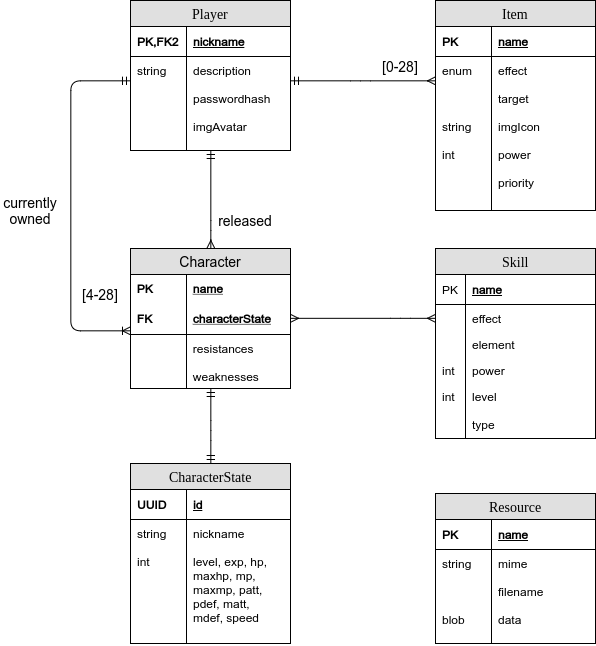
\includegraphics[width=0.5\textwidth]{ERM}
\label{fig:erm}
\end{figure}

\begin{figure}
\caption{Sequenzdiagramm für die Zurücknahme einer Einladung. Simon stellt den Server dar, Alice und Bob die beiden Spieler. Quelle: eigene Darstellung}
\centering
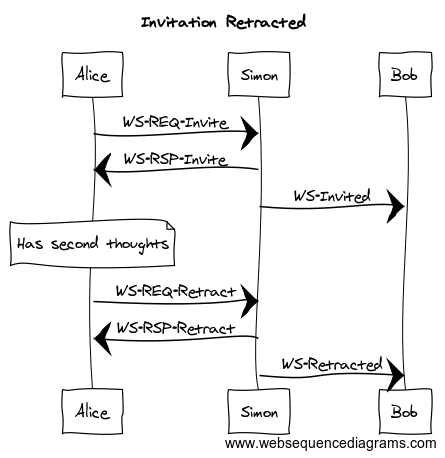
\includegraphics[width=0.5\textwidth]{InvitationRetracted}
\end{figure}

\begin{figure}
\caption{Sequenzdiagramm für die Ablehnung einer Einladung. Simon stellt den Server dar, Alice und Bob die beiden Spieler. Quelle: eigene Darstellung}
\centering
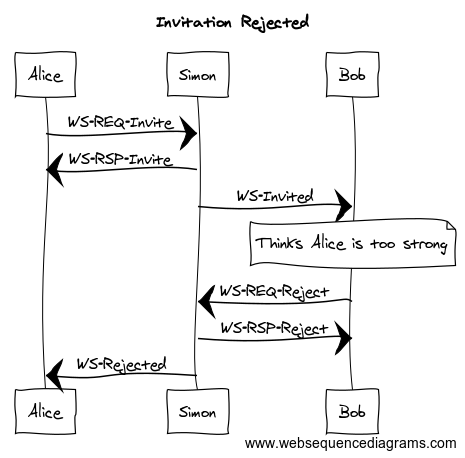
\includegraphics[width=0.5\textwidth]{InvitationRejected}
\end{figure}

\begin{figure}
\caption{Sequenzdiagramm für die Annahme einer Einladung. Simon stellt den Server dar, Alice und Bob die beiden Spieler. Nach Annahme der Einladung wird ein rundenbasiertes Spiel ausgetragen. Quelle: eigene Darstellung}
\centering
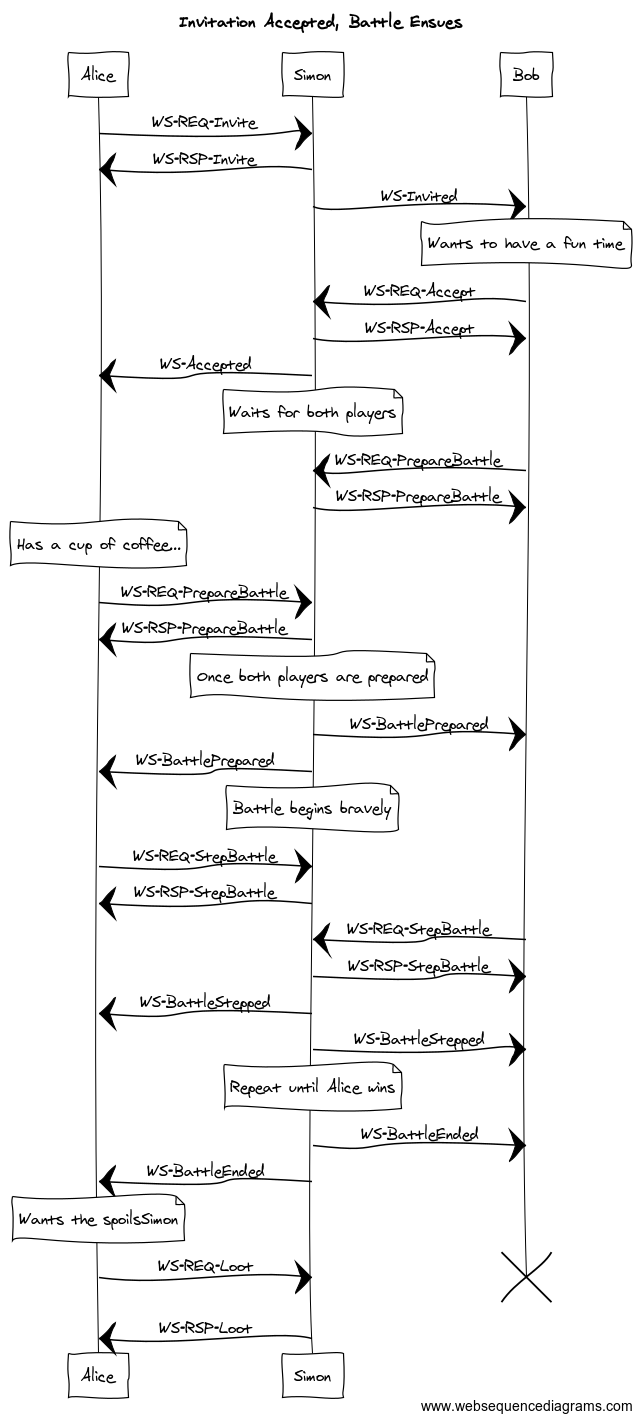
\includegraphics[width=0.5\textwidth]{InvitationAccepted}
\end{figure}

\begin{figure}
\caption{Architektur der entwickelten Software auf Client-Seite. Pfeile stellen Vererbung beziehungsweise Komposition dar. Quelle: eigene Darstellung}
\centering
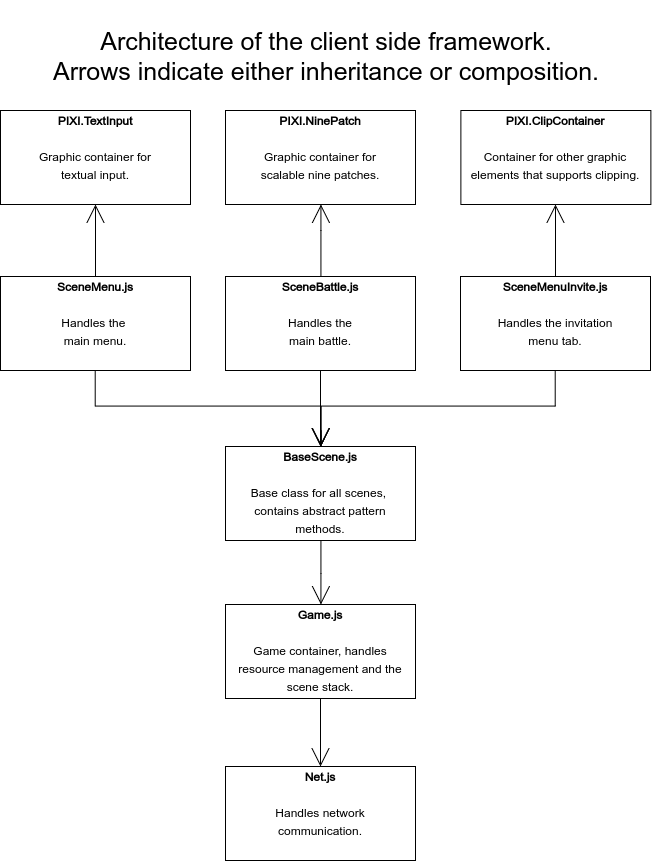
\includegraphics[width=0.7\textwidth]{ClientFramework}
\label{fig:clientarch}
\end{figure}

\begin{figure}
\caption{Menüszene des Spiels. Hier kann der Spieler seinen Status einsehen.}
\centering
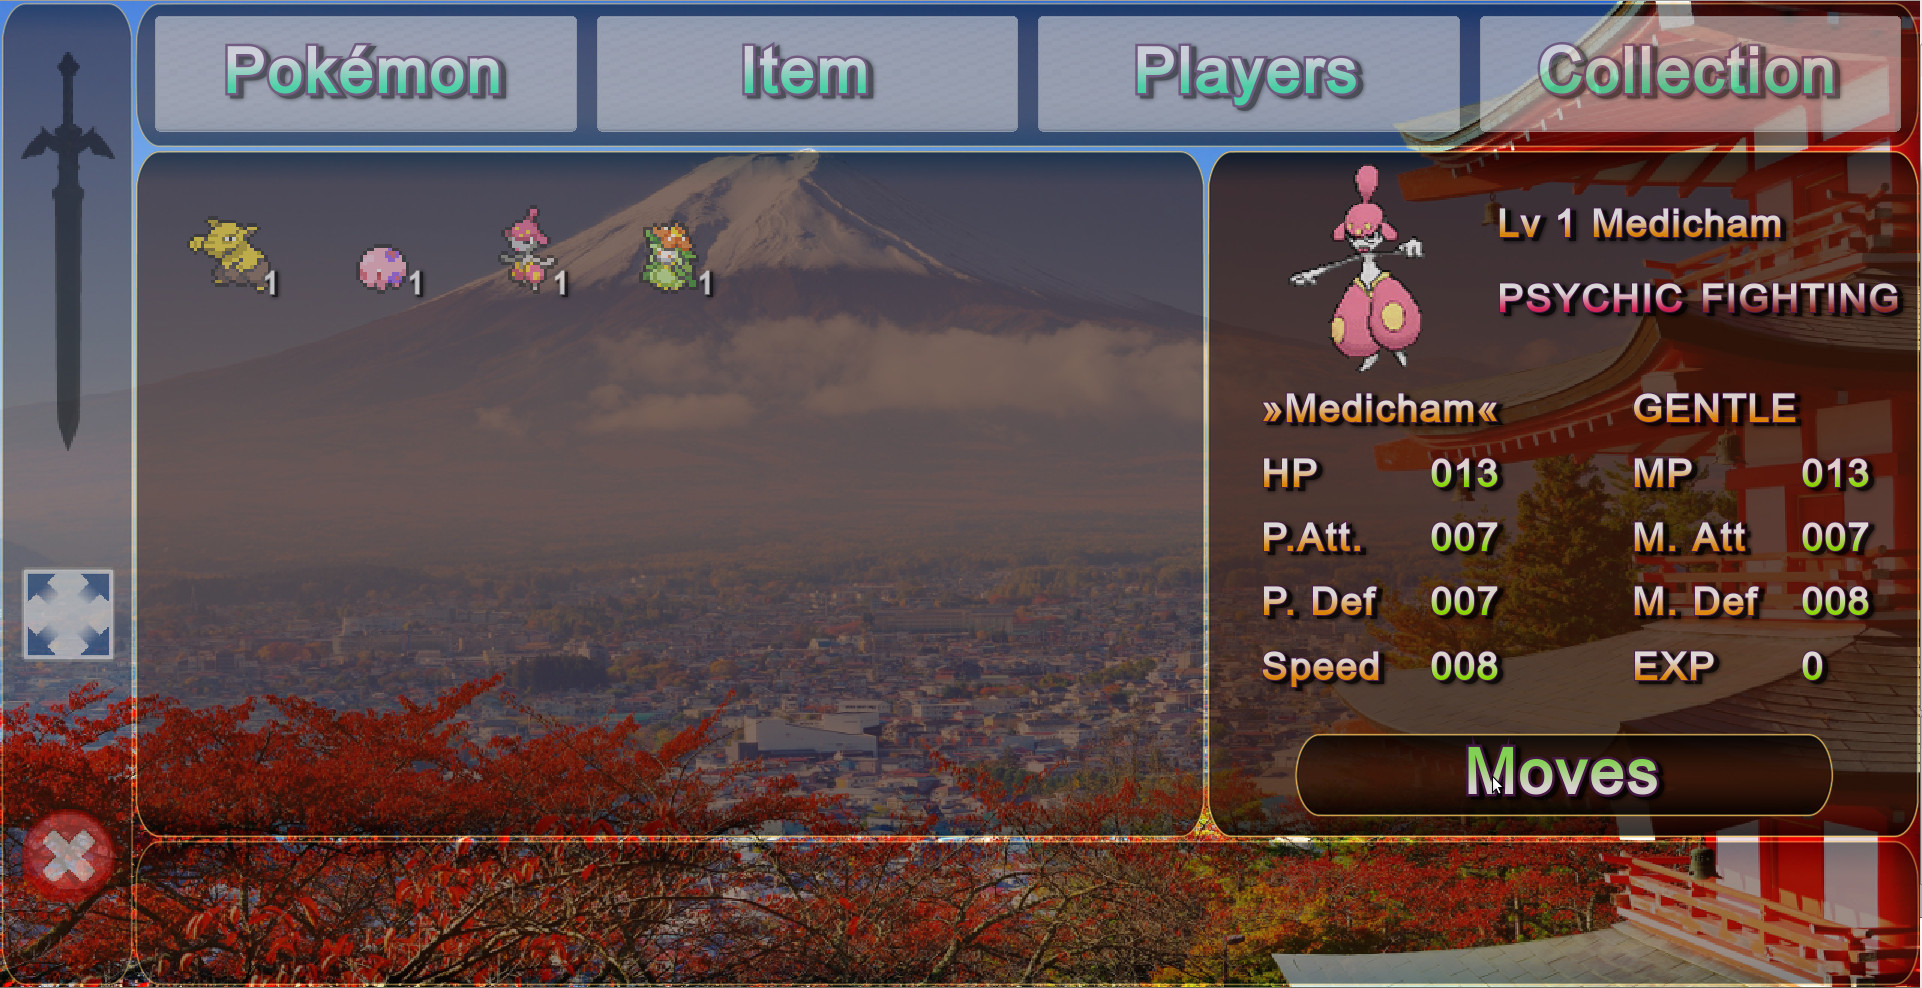
\includegraphics[width=1.0\textwidth]{screenshot1}
\label{fig:scenemenu}
\end{figure}

\begin{figure}
\caption{Kampfzene des Spiels. Hier kann der Spieler seinen Spaß haben.}
\centering
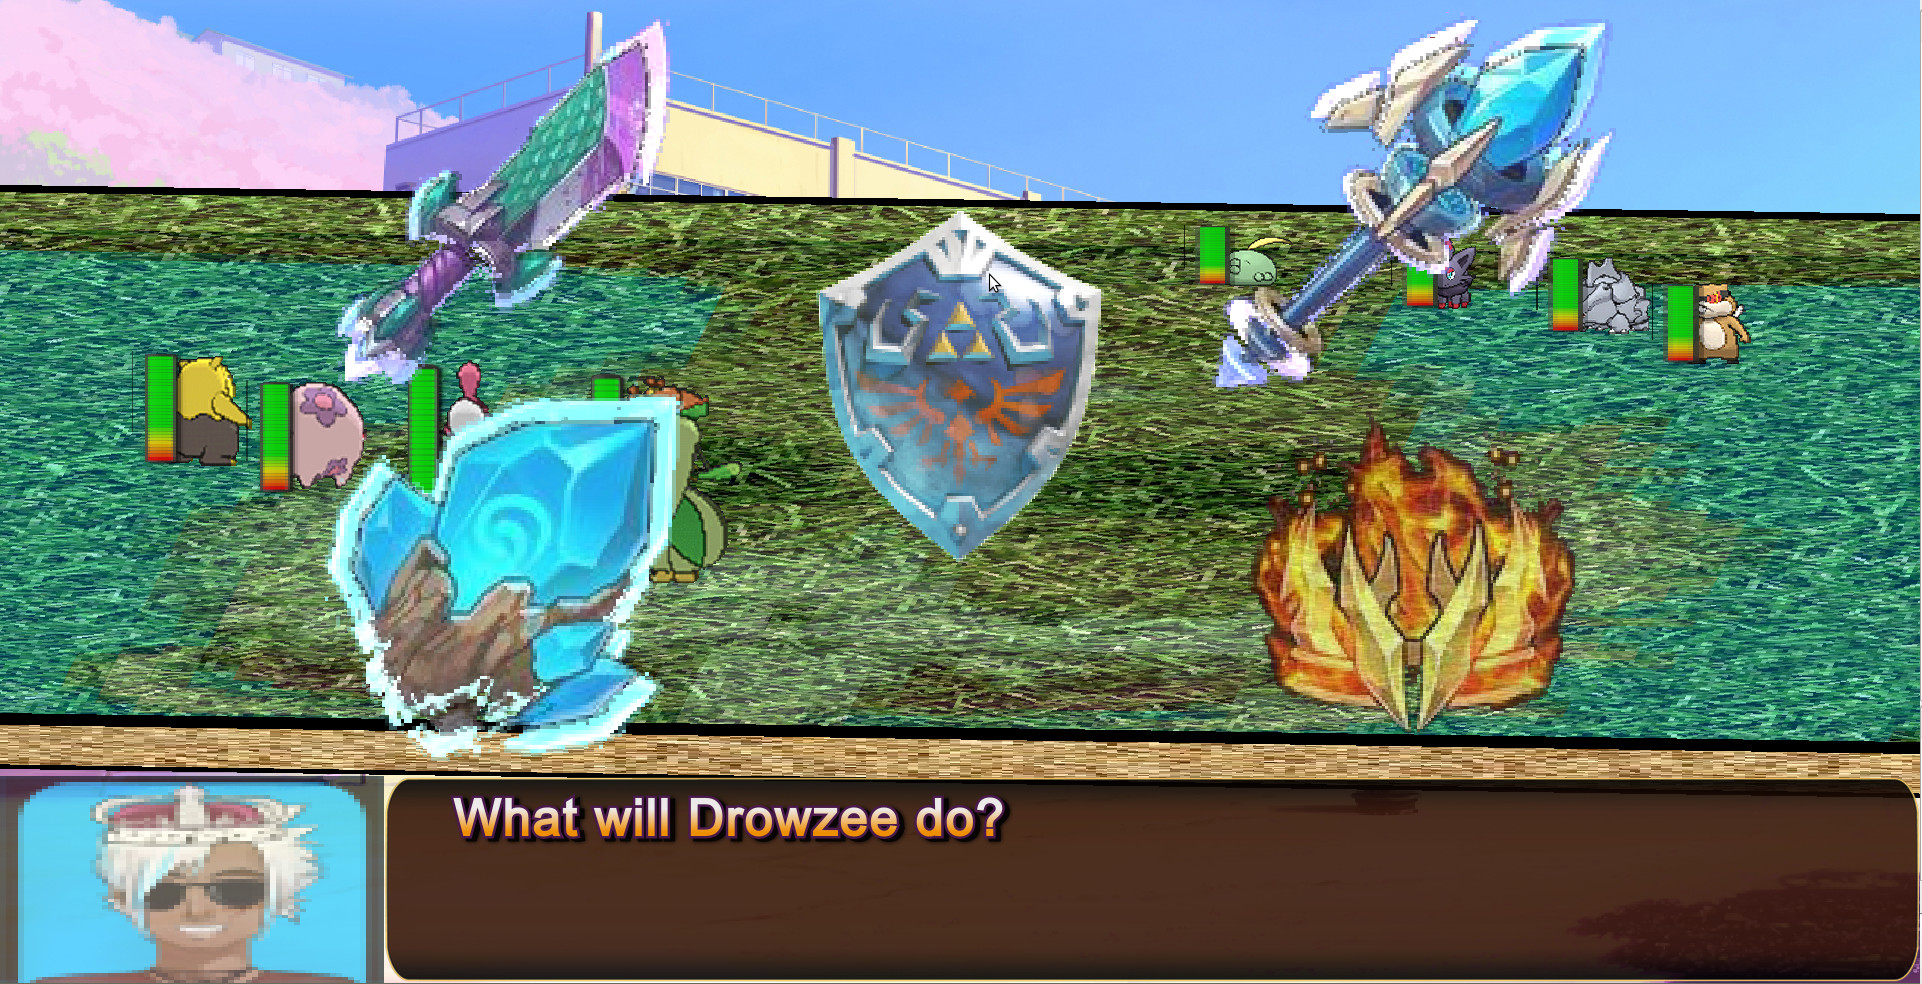
\includegraphics[width=1.0\textwidth]{screenshot2}
\label{fig:scenemenu}
\end{figure}

%%%----------------------------------------------------------
%%%\MakeBibliography
%%%----------------------------------------------------------

\end{document}
